\documentclass{article}
\usepackage[top=1in, bottom=1in, left=1in, right=1in]{geometry}
% \usepackage{fullpage, fancyhdr}
\usepackage{fullpage}
\usepackage{float}
\usepackage{mathtools}
\usepackage{caption}
\usepackage{subcaption}
\usepackage{portland}
\usepackage{graphicx}
%\usepackage{setspace}
\setlength{\topmargin}{0.0in}
\setlength{\headheight}{0.5in}
\setlength{\headsep}{0in}
\setlength{\footskip}{9pt}
\usepackage{listings}
\usepackage{color}


% \pagestyle{fancyplain}
\pagestyle{myheadings}
\voffset=-0.50in
\topmargin=0.00in 
\headsep=0.25in 
\evensidemargin=0in 
\oddsidemargin=0in 
\textwidth=6.6in 
\textheight=10.0in 

\renewcommand{\topfraction}{0.9}	% max fraction of floats at top
\renewcommand{\bottomfraction}{0.8}	% max fraction of floats at bottom
%   Parameters for TEXT pages (not float pages):
\setcounter{topnumber}{2}
\setcounter{bottomnumber}{2}
\setcounter{totalnumber}{4}     % 2 may work better
\setcounter{dbltopnumber}{2}    % for 2-column pages
\renewcommand{\dbltopfraction}{0.9}	% fit big float above 2-col. text
\renewcommand{\textfraction}{0.07}	% allow minimal text w. figs
%   Parameters for FLOAT pages (not text pages):
\renewcommand{\floatpagefraction}{0.7}	% require fuller float pages
% N.B.: floatpagefraction MUST be less than topfraction !!
\renewcommand{\dblfloatpagefraction}{0.7}	% require fuller float pages
% remember to use [htp] or [htpb] for placement

\title{Assignment \# 3: MEMS Transmissibility Calculations}
\date{2/11/2013}
\author{Brian Arnberg}

\markright{Brian Arnberg\hfill ELEC 6760 - Solid State Sensors\hfill}     
\setlength{\parindent}{0pt}


\begin{document}\label{start}

% \begin{titlepage}
% 	\maketitle
% 	\thispagestyle{empty}
% \end{titlepage}


\section*{ Homework Assignment \#3 - Due Mon. 2/11/13 }
\subsection*{ Problem 1 }
Consider the plot in Figure~\ref{fig:plot1}.
\begin{figure}[h]
   \centering
   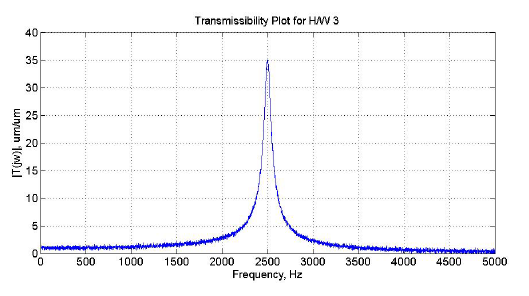
\includegraphics[width=0.95\textwidth,keepaspectratio]{plot1}
   \caption{ This is the transmissibility plot for a MEMS device with a 100$\mu$g proof mass.} 
   \label{fig:plot1}
\end{figure}
\renewcommand{\labelenumi}{\alph{enumi}.}
\begin{enumerate}
	\item What is Q?\\
		$ \max \| T(j\omega) \| \colon Q \gg 1 \colon \omega = \omega_{\text{n}} 
		\Rightarrow Q = 35 \mu m /\mu m $
	\item What is the damping ratio?\\
		$ \zeta = \frac{1}{2 Q} = \frac{1}{2 * 35} = 0.0143 = 14.3 \times 10^{-3} $
	\item What is the natural frequency in KHz?\\
		$ \max \| T(j\omega) \| \colon Q \gg 1 \colon \omega = \omega{\text{n}}
		\Rightarrow \frac{\omega_{\text{n}}}{2\pi} = 2.5 \text{KHz} $
	\item What is the spring constant?\\
		$ {\omega_{\text{n}}}^2 = \text{K} / m
		\Rightarrow \text{K} = {\omega_{\text{n}}}^2 * m
		= (2*\pi*2500 \text{rad/s})^2 (100 \times 10^{-9} kg) = 24.67\text{ }kg/s^2
		= 24.67\text{ N}/m $
	\item What is the damping coefficient?\\
		$ \frac{\omega_{n}}{Q} = \frac{C}{m} 
		\Rightarrow C = \frac{\omega_n m}{Q} 
		= \frac{(2*\pi*2500 \text{HZ})( 100 \times 10^{-9} kg)}{35}
		= 44.88 \times 10^{-6} \text{N}\cdotp s /m $ 
	\item If the device is excited with a sinusoidal input at its natural frequency with an\\
   	amplitude of 0.2$\mu$m, what is the amplitude of the proof mass displacement at that\\
   	frequency?\\
		$ \omega = \omega_n \colon y(t) = A \sin (\omega t) \colon x(t) = B \sin (\omega t) $\\
		$ Q = \max \| T(j\omega) \| = X(s) / Y(s) \rightarrow X(s) = Q \times Y(s) 
		\Rightarrow B = Q \times A $ \\
		$ A = 0.2\mu m \Rightarrow B = 35 \times 0.2 \mu m = 7 \mu m $
	\item For the input in (f), what is the maximum accelertion experienced by the proof\\
		mass, in G's? [1G$ = 9.8 m/s^2$]\\
		$ x(t) = B \sin (\omega t); \dot{x}(t) = B \omega \cos(\omega t); 
		\ddot{x}(t) = -B \omega^2 \sin(\omega t); \max{\ddot{x}} = B {\omega_n}^2$\\
		$\Rightarrow \max{\ddot{x}} = (7 \mu m )(2*\pi*2.5Krad/s)^2 = 1727  m/s^s$\\
		$ 1727 m/s^2 \approx 176.24 G \Rightarrow \max{\ddot{x}} = 176.24 G$

	\item What is the expression for T(s) for this device?\\
		$ T(s) = \frac{2\zeta\omega_n s + {\omega_n}^2}{s^2 + 2\zeta\omega_n s + {\omega_n}^2}
		\colon\colon \zeta = 14.3 \times 10^{-3} \colon \omega_n = 2*\pi*2.5\text{Krad/s}$\\
		$\Rightarrow T(s) = \frac{2 (14.3\times 10^{-3})(2*\pi*2.5Krad/s)(s) + (2*\pi*2.5Krad/s)^2}{
			s^2 + 2 (14.3\times 10^{-3})(2*\pi*2.5Krad/s)(s) + (2*\pi*2.5Krad/s)^2}$\\
		$ T(s) = \frac{449.24 \text{Krad/s} s + 246.7\times 10^6 {\text{rad/s}}^2}{
			s^2 + 449.24 \text{Krad/s} s + 246.7\times 10^6 {\text{rad/s}}^2}$
	\item Using Matlab with an m-file, plot $\|T(j\omega)\|$. 
		Turn in your plot (in a similar format to
   		the one above (it should look very similar, but with less noise)) AND your m-file.\\

\begin{figure}[h]
   \centering
   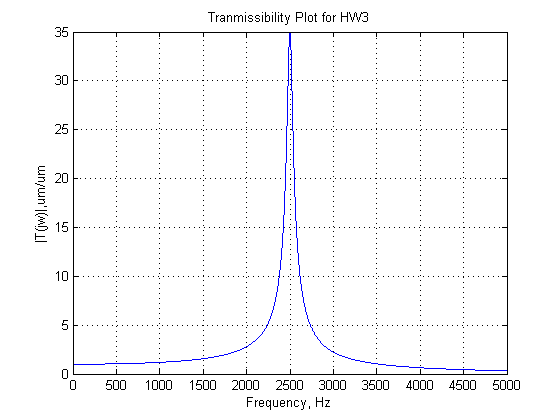
\includegraphics[width=0.95\textwidth,keepaspectratio]{HW3_plot}
   \caption{ This is the plot of $\|T(j\omega)\|$ produced in MATLAB. }
   \label{fig:HW3_plot}
\end{figure}
\lstinputlisting[language=Matlab,numbers=left,frame=single,stepnumber=1,title=\lstname]{HW3_1_i.m}


\end{enumerate}


%  \begin{figure}[htbp]
%   \centering
%   \includegraphics[width=4.0in,keepaspectratio]{E-Field}
%   \caption{\small{ The E-Field pattern produced by the initial code. }}
%   \label{fig:E-Field}
%   \end{figure}
%  \begin{figure}[htbp]
%   \centering
%   \includegraphics[width=4.0in,keepaspectratio]{Power}
%   \caption{\small{ The normalized power pattern of the system.  }}
%   \label{fig:Power}
%   \end{figure}

\label{end}\end{document}


